\documentclass[xcolor ={table,usenames,dvipsnames}]{beamer}
\usepackage[italian]{babel}
\usepackage{color}
\usepackage{txfonts}
\PassOptionsToPackage{dvipsnames}{xcolor}
\title[NN and Statistical Models]{Neural Networks and Statistical Models\\ A Java Implementation}
\author{Alex Foglia}
\institute{Universit\`a  degli Studi di Firenze}
\date{30/01/2019}
%\usepackage{sansmathaccent}
\usetheme{Berlin} 
\useinnertheme{rounded}
\useoutertheme{miniframes} 
\setbeamercovered{dynamic}
\theoremstyle{definition}
\newtheorem{definizione}{Definizione}
\usepackage{tikz}
\usetikzlibrary{arrows}
\usepackage{subfigure}
\usepackage{listings}
\definecolor{codegreen}{rgb}{0,0.6,0}
\definecolor{codegray}{rgb}{0.5,0.5,0.5}
\definecolor{codepurple}{rgb}{0.58,0,0.82}
\definecolor{backcolour}{rgb}{0.95,0.95,0.92}

\lstdefinestyle{mystyle}{
	backgroundcolor=\color{backcolour},   
	commentstyle=\color{codegreen},
	keywordstyle=\color{magenta},
	numberstyle=\tiny\color{codegray},
	stringstyle=\color{codepurple},
	basicstyle=\tiny,
	breakatwhitespace=false,         
	breaklines=true,                 
	captionpos=b,                    
	keepspaces=true,                 
	numbers=left,                    
	numbersep=5pt,                  
	showspaces=false,                
	showstringspaces=false,
	showtabs=false,                  
	tabsize=2
}
\lstset{style=mystyle}
\lstset{language=Java}
\begin{document}
	\begin{frame}
		\maketitle
	\end{frame}
	\begin{frame}{Artificial Neural Networks}
	\begin{itemize}
		\item Artificial Neural Networks (NN) are a wide class of regression models, data reduction models, \emph{nonlinear} dynamical systems
		\item \emph{Computational model} composed of a set of \emph{neurons} which aims to simulate a biological Neural Network
		\item Neurons consist in interconnected computing elements and they are often organized into \emph{layers} 
	\end{itemize}
\end{frame}
\begin{frame}{Example of a NN}
\begin{figure}
	\centering
	{\begin{tikzpicture}[->,>=stealth',shorten >=1pt,auto,node distance=2cm,
		thick,main node/.style={circle,draw,font=\sffamily\Large\bfseries}]
		
		\node[main node] (1) {X};
		\node[main node] (2) [below left of=1] {$n_{1,0}$};
		\node[main node] (3) [right of=2] {$n_{1,1}$};
		\node[main node] (4) [right of=3] {$n_{1,2}$};
		\node[main node] (5) [below of=2]{$n_{2,0}$};
		\node [main node] (6) [below of =4]{$n_{2,1}$};
		\node [main node] (7) [below right of=5]{Y};
		\path[every node]
		
		(1) edge [right] node[left] {} (2)
			edge [right] node[left] {} (3)
			edge [right] node[left] {} (4)
		(2) edge [right] node[left] {} (5)
		(2) edge [right] node[left] {} (6)
		(3) edge [right] node[left] {} (5)
		(3) edge [right] node[left] {} (6)
		(4) edge [right] node[left] {} (5)
		(4) edge [right] node[left] {} (6)
		(5) edge [right] node[left] {} (7)
		(6) edge [right] node[left] {} (7);
		
		\end{tikzpicture}}

\end{figure}
\end{frame}
\begin{frame}{A bit of history}
\begin{itemize}
	\item \emph{Artifical Intelligence} (AI) is a discipline belonging to computer science which studies the theoretical foundations, the methodologies and the techniques that allow computer systems to provide services which would seem to be an exclusive pertinence to human intelligence, for the common observer.
	\footnotesize {[Marco Solmavico]}
\end{itemize}
\end{frame}
\begin{frame}{A bit of history}
\begin{itemize}
	\item In the past, artificial intelligence was based on the intensive use of computing capabailities provided by computer systems
	\item NN is a "novel" approach which aims, through the use of statistical models, to reproduce the concept of "learning"
	\item The alleged "intelligence" of a NN is a matter of dispute, since networks are capable of processing vast amounts of data and making prediction, only as an appropriate statistical model is able to "fit" a sample of observed data
\end{itemize}
\end{frame}
\begin{frame}{NN vs Statistical Models}
\tiny
	\begin{center}
	\begin{tabular}{|c|c|}
	\hline 
	\textbf{Statistical Jargon} & \textbf{NN Jargon} \\ 
	\hline 
	Variables & Features \\ 
	\hline 
	Independent Variable & Inputs \\ 
	\hline 
	Predicted Values & Outputs \\ 
	\hline 
	Dependent Variables & Targets \\ 
	\hline 
	Residual & Errors \\ 
	\hline 
	Estimation & Training, Learning \\ 
	\hline 
	Estimation Criterion & Error Function \\ 
	\hline 
	Observations & Patterns \\ 
	\hline 
	Parameter Estimates & Synaptic Weights \\ 
	\hline 
	Interactions & Higher-Order neurons \\ 
	\hline 
	Transformations & Functional Links \\ 
	\hline 
	Regression & Supervised Learning \\ 
	\hline 
	Data reduction & Unsupervised Learning \\ 
	\hline 
	Cluster Analysis & Competitive Learning \\ 
	\hline 
	Interpolation and Extrapolation & Generalization \\ 
	\hline 
\end{tabular}
\end{center}
\footnotesize
Terms like \emph{sample} and \emph{population} does not have NN equivalents, but data are often divided into a \emph{training set} and \emph{test set} for cross-validation.
\end{frame}
\begin{frame}{NN and Linear Regression Model}
\begin{itemize}
	\item Linear regression models are simple statistical models used to predict the exepcted value of a dependant variable \textbf{Y} given a set of observed variables \textbf{X}
	\item The model is the following:
	$$
	\textbf{Y}_i = \beta_0 + \beta_1 \textbf{X}_i + \epsilon_i
	$$
	\item Such a model identifies a data-fitting \emph{line} 
\end{itemize}
\end{frame}
\begin{frame}{NN and Linear Regression Model}
\begin{itemize}
	\item How to estimate $\beta_0,\beta_1$ parameters?
	\item \color{red} Ordinary least square \color{black} method
	\item $S$ is defined as:
	$$
	S(\beta_0,\beta_1) = \sum_{i=1}^N (y_i - \beta_0 - \beta_1 \textbf{X}_i)^2
	$$
	$S$ is a function from $\mathbb{R}^2 \rightarrow \mathbb{R}$ and parameters $\beta_0,\beta_1$ are estimated  as the arguments of $S$ on which the function evaluates to its minima
\end{itemize}
\end{frame}
\begin{frame}{NN and Linear Regression Model}
	\begin{figure}[h!]
	\centering
	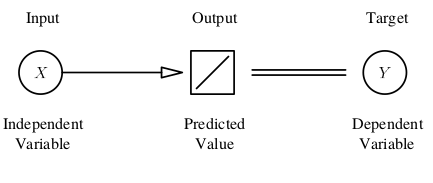
\includegraphics[scale=2.5]{../Relazione/img/linreg}
\end{figure}
\end{frame}
\begin{frame}{NN and Logistic Regression Model}
\begin{itemize}
	\item A perceptron is a very small NN which usually computes a linear combination of the inputs
	\item A perceptron has $n>0$ input
	\item Each input has a specific \emph{weight} $\beta_i$
	\item The \emph{weights} are the parameters to be estimated, moreover the parameters the model has to \emph{learn}
\end{itemize}
\end{frame}
\begin{frame}{NN and Logistic Regression Model}
\begin{itemize}
	\item More generally, the output of a perceptron is an evaluation of an \emph{activation function} on the provided inputs
	\item Activation functions are usually \emph{bounded}
	\item A bounded function maps any real input to a bounded range. Bounded activation functions are called \emph{squashing functions}, for instance the logistic function:
	$$
	\texttt{act}(x) = \dfrac{1}{1+e^{-x}}
	$$
	Is a bounded activation function which maps any real argument into the range $(0,1)$
\end{itemize}
\end{frame}
\begin{frame}{NN and Logistic Regression Model}
\begin{itemize}
	\item What a perceptron is supposed to do is, given $\textbf{x}$ as an input, and assuming the logistic function as the activation function:
	\begin{itemize}
		\item Compute $$\hat x = \sum_{i=1}^N \beta_i \textbf{X}_i$$
		\item Return \texttt{act}$(\hat x) =$ $$ \dfrac{1}{1+e^{-(\beta_1\textbf{X}_1+ \dots + \beta_n\textbf{X}_n)}}$$
	\end{itemize}
\item Notice that 
$$
\dfrac{1}{1+e^{-(\beta_i\textbf{X}_i+ \dots + \beta_n\textbf{X}_n)}} =\dfrac{e^{(\beta_i\textbf{X}_i+ \dots + \beta_n\textbf{X}_n)}}{1+e^{(\beta_i\textbf{X}_i+ \dots + \beta_n\textbf{X}_n)}}
$$
\end{itemize}
\end{frame}
\begin{frame}{NN and Logistic Regression Model}
\begin{itemize}
	\item The \emph{logisitc regression model} is a \emph{non-linear} regression model used when the dependent variable is dichotomic
	\item The model formula is the following:
	$$
	\mathbb{E}(\textbf{Y}|\textbf{X}) = \dfrac{e^{\beta_0 + \beta_1x_1+\dots+\beta_n x_n}}{1 +e^{\beta_0 + \beta_1x_1+\dots+\beta_n x_n} }
	$$
	\item That is, exactly, what a perceptron with a logistic activation function computes
\end{itemize}
\end{frame}
\begin{frame}{NN and Logistic Regression Model}
\begin{itemize}
	\item Again, how to estimate $\beta_i$ parameters?
	\item Two possible ways:
	\begin{itemize}
	\item \color{red} Maximum likelihood \color{black} method
	\item \color{red} Gradient descent \color{black} method
	\end{itemize}
	\item The gradient descent method is an optimization algorithm which aims to estimate parameters given a set of pairs\\*\texttt{input - expected output} (the training set)
\end{itemize}
\end{frame}
\begin{frame}{NN and Logistic Regression Model}
\begin{itemize}
	\item The goal here is to minimize 	$$
	\sum \sum r_j^2
	$$
	\item	Where the $r_j$ is the difference between the expected output and the predicted value
	\item This is why estimation and learning are the same concept as perceived from different points of view
\end{itemize}
\end{frame}
\begin{frame}{NN and Logistic Regression Model}
	\begin{figure}[h!]
	\centering
	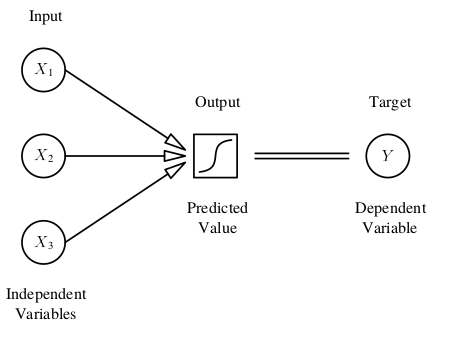
\includegraphics[scale=2.4]{../Relazione/img/logreg}
\end{figure}
\end{frame}
\begin{frame}{NN and Nonlinear Regression Models}
\begin{itemize}
	\item Neurons are often organized into \emph{layers}
	\item NN seen before are simple perceptrons composed of two layers: the input layer and the output layer
	\item If it is introduced another \emph{hidden} layer between input and output, you obtain a multi-layer perceptron (MLP)
\end{itemize}
\end{frame}
\begin{frame}{NN and Nonlinear Regression Models}
\begin{itemize}
	\item 
	If the model includes estimated weights between the inputs and the hidden layer, and the hidden layer uses nonlinear activation functions, the model becomes nonlinear:
	\begin{figure}[h!]
		\centering
		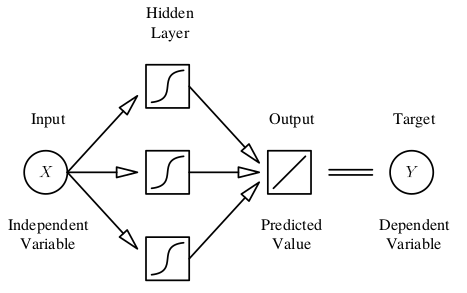
\includegraphics[scale=2]{../Relazione/img/nonlinreg}
	\end{figure}
\end{itemize}
\end{frame}
\begin{frame}{NN and Nonlinear Regression Models}
\begin{itemize}
	\item This is a simple MLP implementing a non linear regression model:
	$$
	\textbf{Y} = f(\textbf{X}) + \textbf{b}
	$$
	\item MLP are general-purpose, flexible, nonlinear models that can approximate
	virtually any function to any desired degree of accuracy
	\item MLP are called \emph{universal approximators} and they can be used when you have little knowledge about the relationship between the independent and dependent variables
\end{itemize}
\end{frame}
\begin{frame}{Linear Regression Implementation}
\begin{itemize}
	\item Start from the linear regression model:
	$$
	\textbf{Y}_i = \beta_0 + \beta_1 \textbf{X}_i + \varepsilon_i
	$$
	\begin{figure}[h!]
		\centering
		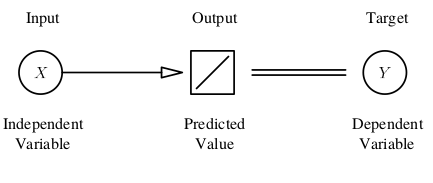
\includegraphics[scale=2]{../Relazione/img/linreg}
	\end{figure}
\end{itemize}
\end{frame}
\begin{frame}[fragile]{Linear Regression Implementation}
\begin{itemize}
	\item Suppose it is $\varepsilon_i = 0$
	\item Consider the following class:
\begin{lstlisting}[language=Java]
public class Neuron {
	private double b0,b1;
	public double predict(double x) {
		return b0 + b1*x;
	}
	public static void main(String[] args) {
		Neuron y = new Neuron();
		System.out.println(y.predict(7));
	}
}
\end{lstlisting}
\end{itemize}
\end{frame}
\begin{frame}{Linear Regression Implementation}
\begin{itemize}
	\item The output provided by the execution of this code is \textit{0.0}, due to the fact that the $\beta_0,\beta_1$ parameters are not yet estimated.
	\item  $\beta_0,\beta_i$ are estimated as the minima of the function
	$$
	S(\beta_0,\beta_1) = \sum_{i=1}^N (y_i - \beta_0 - \beta_1 x_i)^2
	$$
	\item It is possible to find the minima by setting
	$\nabla S = 0$
	$$
	\frac{\vartheta S}{\vartheta \beta_0} = -2 \sum_{i=1}^N (y_i - \beta_0 - \beta_1x_i) = 0,\;
	\frac{\vartheta S}{\vartheta \beta_1} = -2 \sum_{i=1}^N (y_i - \beta_0 - \beta_1 x_i) x_i = 0
	$$
	$$
	\beta_1 = \frac{\sigma(x,y)}{\sigma^2(x)},\;\;\;\;
	\beta_0 = \overline y - \beta_1 \overline x
	$$
\end{itemize}
\end{frame}
\begin{frame}[fragile]{Linear Regression Implementation}
	Extend the class code:
	\begin{lstlisting}[language = Java]
public void estimateParameters(double[] xi, double[] yi) {
	b1 = var(xi,yi) / var(xi,xi);
	b0 = mean(yi) - b1*mean(xi);
}
private double mean(double[] v) {
	double m = 0;
	for(int i=0; i<v.length;i++) {
		m+=v[i];
	}
	return m/v.length;
}
private double var(double[] x, double[] y) {
	double var = 0;
	double mx = mean(x);
	double my = mean(y);
	for(int i=0; i<x.length;i++) {
		var+= (x[i]-mx)*(y[i]-my);
	}
	return var/x.length;
}
\end{lstlisting}
\end{frame}
\begin{frame}[fragile]{Linear Regression Implementation}
Suppose it exists a sample \textbf{X} for which it is known that all the values of the dependent variable \textbf{Y} are on the bisector of the second quadrant of the Cartesian plane:
$$
\textbf{X} = \{X_i\} = \{1,2,3,4,5\}
\;\;
\textbf{Y} = \{Y_i\} = \{1,2,3,4,5\}
$$
\begin{lstlisting}[language = Java]
Neuron y = new Neuron();
y.estimateParameters(new double[]{1,2,3,4,5}, new double[]{1,2,3,4,5});
System.out.println(y.predict(7));
System.out.println("Y=" + y.b0 + "+" + y.b1+"X");
\end{lstlisting}
\begin{lstlisting}
7.0
Y = 0.0 + 1.0X
\end{lstlisting}
\end{frame}
\begin{frame}[fragile]{Linear Regression Implementation}
\begin{itemize}
\item As it is expected, even if in the \emph{training set} does not appear the expected output for value $7$, our linear regression model is able to predict the output for such a value: \textit{7.0}
\item In fact the regression line is exactly the requested identity function
\end{itemize}
\end{frame}
\begin{frame}[fragile]{Extending the code: Logistic Regression}
The code must be modified in order to implement a logistic regression model:
\begin{lstlisting}[language=Java]
public class Neuron {
	private double[] weights;

	public Neuron(int n_inputs) {
		weights = new double[n_inputs];
	}

	private double logistic(double x) {
		return 1 / (1 + Math.exp(-x));
	}

	public double predict(double[] inputs) {
		double sum = 0;
		for (int i = 0; i < inputs.length; i++) {
			sum += weights[i] * inputs[i];
		}
		return logistic(sum);
	}
}
\end{lstlisting}
\end{frame}
\begin{frame}[fragile]{Extending the code: Logistic Regression}
Now the job is to modify the \texttt{estimateParameter()} method seen before in order to estimate weights using the gradient descent method:
\begin{lstlisting}[language=Java]
public void estimateParameters(double[][] xi, double[] yi) {
	double[] gradient = new double[weights.length];
	for (int i = 0; i < xi.length; i++) {
		for (int j = 0; j < xi[0].length; j++) {
				gradient[j] += xi[i][j] * (yi[i] - predict(xi[i]));
		}
	}
	for (int j = 0; j < weights.length; j++)
		weights[j] += gradient[j];
}
\end{lstlisting}
Note that the logistic function has a "friendly" derivative that permit us to compute its gradient in such an easy way
\end{frame}
\begin{frame}[fragile]{Extending the code: Logistic Regression}
Consider this piece of python code:
\begin{lstlisting}[language=Python]
import math
b0 = -1
b1 = -2
squash = lambda x: math.exp((b0*x[0]+b1*x[1]))/(1+math.exp((b0*x[0]+b1*x[1])))
print squash([1,0])
print squash([0,1])
print squash([0,0])
print squash([1,1])
\end{lstlisting}
Executing it, it is possible to generate data from the logistic function:
$$
f(\textbf x) = \frac{e^{-x_1-2x_2}}{1+e^{-x_1-2x_2}},
$$
\end{frame}
\begin{frame}[fragile]{Extending the code: Logistic Regression}
It is possible now to train this simple network with such data:
\begin{lstlisting}[language=Java]
Neuron n = new Neuron(2);
double[][] in = {{1,0},{0,1},{0,0},{1,1}};
double[] out = {0.2689414213699951,0.11920292202211755,0.5,0.04742587317756679};
for(int i=0; i<10000;i++)
	n.estimateParameters(in, out);
System.out.println(Arrays.toString(n.weights));
\end{lstlisting}
Obtaining the following coefficients:
\begin{lstlisting}
[-1.0000000000000004, -1.9999999999999993]
\end{lstlisting}
Which are approximately the $\beta_0,\beta_1$ used to generate data
\end{frame}
\begin{frame}{The XOR operator}
Consider the following \emph{truth table}:
\begin{center}
	\begin{tabular}{|c|c|c|}
		\hline 
		$x_1$ & $x_2$ & $x_1$ $\oplus$ $x_2$ \\ 
		\hline 
		0 & 0 & 0 \\ 
		\hline 
		0 & 1 & 1 \\ 
		\hline 
		1 & 0 & 1 \\ 
		\hline 
		1 & 1 & 0 \\ 
		\hline 
	\end{tabular}
\end{center} 
This is known as the logical operator \textit{xor}. A NN composed of a nonlinear MLP is capable to learn the \textit{xor} computation.
\end{frame}
\begin{frame}{From Logistic Regression to Universal Approximators}
\begin{figure}[h]
	\centering
	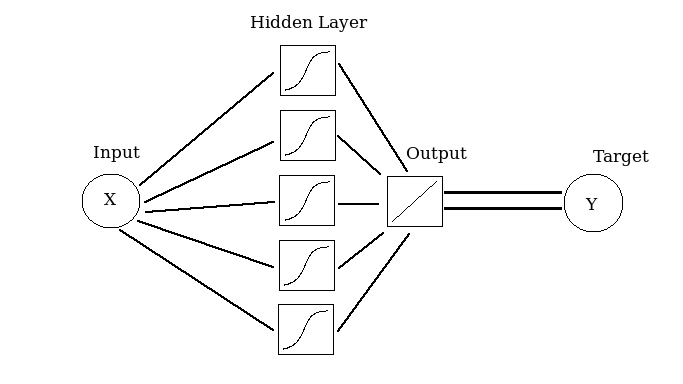
\includegraphics[scale=0.35]{../Relazione/img/mymodel}
	\label{fig:mymodel}
\end{figure}
This is a MLP, or \emph{universal approximator}. The aim is to modify the provided code in order to implement such a MLP  able to learn to compute the \emph{xor}.
\end{frame}
\begin{frame}[fragile]{From Logistic Regression to Universal Approximators}
Start from the Neuron class:
\begin{lstlisting}[language=Java]
public class Neuron {
	public double[] weights;
	public double[] inputs;
	public double output;
	public Neuron(int n_inputs) {
		weights = new double[n_inputs];
		for(int i = 0; i < n_inputs; i++){
			weights[i] = Math.random();
		}
	}
	private double logistic(double x) {
		return 1/(1+Math.exp(-x));
	}
	public double predict(double[] inputs) {
		this.inputs = inputs;
		double sum = 0;
		for(int i=0; i<inputs.length;i++) {
			sum += inputs[i] * weights[i];
		}
		this.output = logistic(sum);
		return output;
	}
}
\end{lstlisting}
\end{frame}
\begin{frame}[fragile]{From Logistic Regression to Universal Approximators}
Since MLPs have more than one layer, we define, from a programming point of view, what a layer is: a collection of Neurons.
\begin{lstlisting}[language=Java]
public class NeuronLayer {
	public Neuron[] neurons;
	public NeuronLayer(int n, int inputsPerNeuron) {
	this.neurons = new Neuron[n];
	for (int i = 0; i < n; i++) {
		this.neurons[i] = (new Neuron(inputsPerNeuron));
	}
	}
	public double[] feedForward(double[] inputs) {
		double[] outputs = new double[neurons.length];
		for (int i = 0; i < neurons.length; i++) {
			outputs[i] = (neurons[i].predict(inputs));
		}
		return outputs;
	}
	public double[] getOutputs() {
		double[] outputs = new double[neurons.length];
		for (int i = 0; i < neurons.length; i++) {
			outputs[i] = neurons[i].output;
		}
	return outputs;
	}
}
\end{lstlisting}
\end{frame}
\begin{frame}[fragile]{From Logistic Regression to Universal Approximators}
Putting layers together means to construct a MLP Neural Network:
\begin{lstlisting}
public class NeuralNetwork {
		private int n_in,n_hid,n_out;
		private NeuronLayer hidden,output;
		public NeuralNetwork(int inputNeurons,int hiddenNeurons,int numberOfOutputs){
			n_in = inputNeurons;
			n_hid = hiddenNeurons;
			n_out = numberOfOutputs;
			hidden = new NeuronLayer(n_hid, n_in);
			output = new NeuronLayer(n_out, n_hid);
		}
	}
}
\end{lstlisting}
The MLP must be capable of performing prediction:
\begin{lstlisting}
public double[] feedForward(double[] inputs) {
	double[] hidden_outputs = hidden.feedForward(inputs);
	return output.feedForward(hidden_outputs);
}
\end{lstlisting}
\end{frame}
\begin{frame}[fragile]{Backpropagation}
Last, the MLP must be capable of being trained in order to estimate neurons weights:
\begin{lstlisting}
public void train(double[] training_in, double[] training_out) {
	feedForward(training_in);
	double[] deltaWrtOut = new double[n_out];
	for (int i = 0; i < n_out; i++) {
		double target_output = training_out[i];
		double actual_output = output.neurons[i].output;
		double deltaWrtInput = -(target_output - actual_output) * actual_output * (1 - actual_output);
		deltaWrtOut[i] = deltaWrtInput;
	}
\end{lstlisting}
\end{frame}
\begin{frame}[fragile]{Backpropagation}
\begin{lstlisting}
	double[] deltaWrtHid = new double[n_hid];
	for(int i=0; i<n_hid;i++) {
		double deltaWrtHiddenOut = 0;
		for(int j=0; j<n_out;j++) {
			deltaWrtHiddenOut+=deltaWrtOut[j] * output.neurons[j].weights[i];
		}
	double actual_output = hidden.neurons[i].output;
	double deltaWrtIn = actual_output * (1 - actual_output);
	deltaWrtHid[i] = deltaWrtHiddenOut * deltaWrtIn;
	}
	for (int i = 0; i < n_out; i++) {
		for (int j = 0; j < n_hid; j++) {
			double act_input = output.neurons[i].inputs[j];
			double deltaWrtWeight = deltaWrtOut[i] * act_input;
			output.neurons[i].weights[j] -= deltaWrtWeight;
		}
	}
	for (int i = 0; i < n_hid; i++) {
		for (int j = 0; j < n_in; j++) {
			double act_input = hidden.neurons[i].inputs[j];
			double deltaWrtWeight = deltaWrtHid[i] * act_input;
			hidden.neurons[i].weights[j] -= deltaWrtWeight;
		}
	 }
}
\end{lstlisting}
\end{frame}
\begin{frame}[fragile]{Error Evaluation}
 Another method is added in order to compute the total network error with respect to a training set:
\begin{lstlisting}
public double totalError(double[][][] training_sets) {
	double err = 0;
	for (int i = 0; i < training_sets.length; i++) {
		double[] t_in = training_sets[i][0];
		double[] t_out = training_sets[i][1];
		double[] act_out = feedForward(t_in);
		for (int j = 0; j < act_out.length; j++) {
			double target_output = t_out[j];
			double actual_output = output.neurons[j].output;
			double squareError = 0.5 * Math.pow(target_output - actual_output, 2);
			err += squareError;
		}
	}
return err;
}
\end{lstlisting}
\end{frame}
\begin{frame}[fragile]{Launch the NN}
Now the model is ready to use. Start from constructing the model shown before. It has 2 inputs, 5 hidden neurons, and 1 output:
\begin{lstlisting}
NeuralNetwork nn = new NeuralNetwork(2, 5, 1);
\end{lstlisting}
Define the training sets as defined in the \emph{xor} table of truth:
\begin{lstlisting}
double[][][] training_sets = {{{0, 0}, {0}},{{0, 1}, {1}},{{1, 0}, {1}},{{1, 1}, {0}}};
\end{lstlisting}
Train the network:
\begin{lstlisting}
System.out.println("Error before training: "+nn.totalError(training_sets));
for (int i = 0; i < 10000; i++) {
	int randIndex = (int) (Math.random() * training_sets.length);
	double[] t_in = training_sets[randIndex][0];
	double[] t_out = training_sets[randIndex][1];
	nn.train(t_in, t_out);
}
System.out.println("Error after training: "+nn.totalError(training_sets));
\end{lstlisting}
And this is the output:
\begin{lstlisting}
Error before training: 0.7825167086789118
Error after training: 0.0019131802708672071
\end{lstlisting}
\end{frame}
\begin{frame}{Launch the NN}
\begin{itemize}
\item What it is implemented is a MLP which performs a \emph{xor} approximation using the statistical model \emph{non-linear regression}
\item  If you try to train the MLP with other datasets which arise from considering other functions than the \emph{xor}, such as the \emph{and}, \emph{nand}, etc, the MLP will approximate them with the same degree of accuracy
\item The entire code is available at:\\* \href{https://github.com/alexfoglia1/MASL/tree/master/exam/JavaNN/src}{https://github.com/alexfoglia1/MASL/tree/master/exam/JavaNN/src}
\end{itemize}
\end{frame}
\end{document}